\chapter{Serverless design patterns} \label{cha:patterns}

In this chapter we take a look at serverless design patterns. Design patterns describe commonly accepted, reusable solutions to recurring problems \parencite{hohpe2004enterprise}. A design pattern is not a one-size-fits-all solution directly translatable into software code, but rather a formalized best practice that presents a common problem in its context along a general arrangement of elements that solves it \parencite{gamma94designPatterns}. The patterns in this chapter are sourced from scientific literature on serverless computing as well as cloud provider documentation \parencite{aws18serverlessLens}. Literature on object-oriented patterns (OOP) \parencite{gamma94designPatterns}, SOA patterns \parencite{rotem12soa} and enterprise integration patterns (EIP) \parencite{hohpe2004enterprise} was also reviewed for applicable practices.

Enterprise integration patterns (EIP), as serverless is all about integrations. \textcite{hohpe2004enterprise} present a number of asynchronous messaging architectures in the seminal book on EIP. While predating the whole serverless phenomenon the patterns are still relevant. Hohpe even demonstrated implementing one of his patterns on top of Google's serverless platform \href{http://www.enterpriseintegrationpatterns.com/ramblings/google_cloud_functions.html}{in a blog post}. E.g. patterns like Idempotent Receiver, Dead-letter Channel as well as the 4 more general integration styles of File Transfer, Shared Database, RPC and Messaging. Many patterns implemented internally by FaaS platforms already!

SOA patterns: as FaaS functions are self-contained nanoservices these might have some relevance. SOA patterns \parencite{rotem12soa} include Saga, Decoupled Invocation and others. As with EIP, some patterns are already implemented by the FaaS platform.

FaaSification: \textcite{spillner17transformpython} describes an automated approach to transform monolithic Python code into modular FaaS units by partially automated decomposition. Doesn't really seem suitable for the web application migration process covered in this thesis but worth mentioning.

\section{Composition patterns} \label{sec:compositionPatterns}

The following patterns concern serverless function composition: how to compose and orchestrate serverless functions together into more extensive sequences or workflows?

\subsection{Routing Function} \label{subsec:routingFunction}

\textbf{Problem:} How to branch out execution flow based on request payload?

\begin{figure}[h]
  \centering
  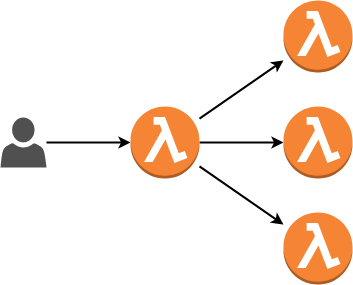
\includegraphics[width=0.4\textwidth]{patterns/routing-function.png}
  \caption{Routing Function}
  \label{fig:patternRoutingFunction}
\end{figure}

\textbf{Solution:} Use a central routing function to receive requests and invoke appropriate functions based on request payload.

This pattern involves instantiating a routing function that contains all the necessary information to route requests to other functions. All function invocations are directed to the routing function, which in turn invokes target functions according to request payload. The routing function finally passes target function return value over to the client.

It's notable that FaaS platforms commonly provide API gateways and other tools for routing, for example the Amazon API Gateway \parencite{awslambda0218}. These tools are however mostly limited to path-based routing, whereas a routing function can be implemented to support more dynamic use cases. Also interestingly, according to an industry survey \parencite{leitner18industrialpractice}, some practicioners opted for the Routing Function pattern over platform API gateway services as they found the latter cumbersome to manage. \textcite{sbarski2017serverless} similarly postulate that the pattern ``can simplify the API Gateway implementation, because you may not want or need to create a RESTful URI for every type of request''. One advantage of the pattern is that the routing function can be used to supplement request payload with additional context or metadata. A centralized routing function also means that all routing configuration is found in one place, and that public-facing API routes only need to be configured for one function, not all of them \parencite{leitner18industrialpractice}.

The pattern's major disadvantage is double billing, as the routing function essentially has to block and wait until the target function finishes execution. Additionally, as routing is implemented at function code level, information about function control flow gets hidden in implementation rather than being accessible from configuration \parencite{leitner18industrialpractice}.

The Routing Function pattern is related to the OOP Command pattern, which is used to decouple caller of the operation from the entity that carries out the processing via an intermediary command object \parencite{gamma94designPatterns}. A related EIP pattern is Content-Based Router, which ``examines the message content and routes the message onto a different channel based on data contained in the message'' \parencite{hohpe2004enterprise}. \textcite{hohpe2004enterprise} caution that the router should be made easy to maintain as it can become a point of frequent configuration.

\subsection{Function Chain} \label{subsec:functionChain}

\textbf{Problem:} Task exceeds maximum function execution duration, resulting in a timeout.

\begin{figure}[h]
  \centering
  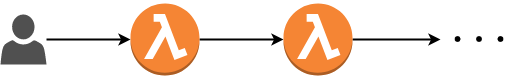
\includegraphics[width=0.5\textwidth]{patterns/function-chain.png}
  \caption{Function Chain}
  \label{fig:patternFunctionChain}
\end{figure}

\textbf{Solution:} Split the task into separate function invocations that are chained together sequentially.

The Function Chain comprises of an initial function and any number of subsequent functions. The initial function begins computation while keeping track of remaining execution time. Foe example in AWS Lambda the execution context contains information on how many milliseconds are left before termination \parencite{awslambda0218}. Upon reaching its duration limit, the initial function invokes another function asynchronously, passing along as parameters any state necessary to continue task computation. Since the intermediary invocation is asynchronous (``fire-and-forget''), the initial function can terminate without affecting the next function in chain.

The Function Chain pattern is in effect a workaround over the duration limit that FaaS platforms place on function execution \parencite{leitner18industrialpractice}. The pattern was reported to be used at least occasionally in an industry study by \textcite{leitner18industrialpractice}. Its disadvantages include strong coupling between chained functions, increase in the number of deployment units and the overhead of transferring intermediate execution state and parameters between each chained function. \textcite{leitner18industrialpractice} also note that splitting some types of tasks into multiple functions can be difficult. Finally, as the pattern relies on asynchronous invocation, the last function in chain has to persist computation result into an external storage for the client to access it, which brings in further dependencies.

\subsection{Fan-out/Fan-in} \label{subsec:FanoutFanin}

\textbf{Problem:} Resource limits on a single function lead to reduced throughput.

% TODO visualize
% \begin{figure}[h]
%   \centering
%   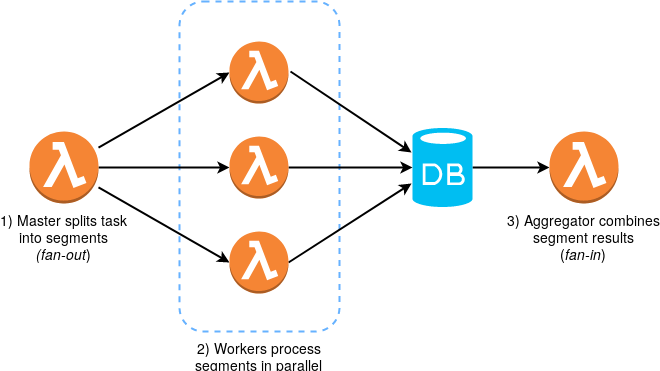
\includegraphics[width=0.4\textwidth]{patterns/fan-out-fan-in.png}
%   \caption{Fan-out/Fan-in}
%   \label{fig:fantOutFanIn}
% \end{figure}

\textbf{Solution:} Split task into multiple parallel invocations.

As discussed, serverless functions are limited in execution duration as well as CPU and memory capacity. The Function Chain pattern (section \ref{subsec:functionChain}) works around the former limitation but is still constrained by a single function's computing resources, which can result in prohibitively slow throughput for compute-intensive tasks. The Fan-out/Fan-in pattern is an alternative approach that takes advantage of serverless platforms' inherent parallelism. The pattern consists of a master function that splits the processing task into segments and then asynchronously invokes a worker function for each segment. Having finished processing, each worker function stores its result on a persistence layer, and finally an aggregator function combines the worker results into a single output value -- although the aggregation step can be omitted in cases where intermediary results suffice. As each worker function invocation runs in parallel with its own set of resources, the pattern leads to faster completion of the overall task. \parencite{zambrano18patterns}

The Fan-out/Fan-in pattern lends itself well to tasks that are easily divisible into independent parts: the efficiency gained depends on the granularity of each subdivision. Conversely, an apparent limitation to the pattern is that not all tasks can be easily distributed into separate worker functions. \textcite{mcgrath16cloudEventParadigms} utilize the pattern in ``easily and performantly solving a large-scale image resizing task''. The authors point out how the pattern reduces development and infrastructure costs compared to a traditional multi-threaded application which ``typically demands the implementation of a queueing mechanism or some form of worker pool''. \textcite{lavoie19efficiency} similarly study ``the efficiency of a serverless architecture for running highly parallelizable tasks'' in comparison to a conventional MapReduce solution running on Apache Spark, concluding that ``the serverless technique achieves comparable performance in terms of compute time and cost''.

\textcite{hohpe2004enterprise} present a similar approach to messaging with the EIP pattern of Composed Message Processor, which ``splits the message up, routes the sub-messages to the appropriate destinations and re-aggregates the responses back into a single message.''

\subsection{State Machine} \label{subsec:stateMachine}

\textbf{Problem:} How to coordinate complex, stateful procedures with branching steps?

\begin{figure}[h]
  \centering
  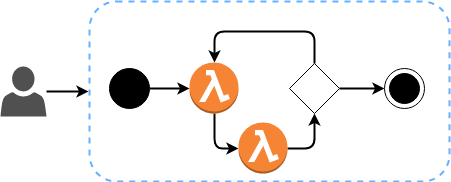
\includegraphics[width=0.6\textwidth]{patterns/state-machine.png}
  \caption{State Machine}
  \label{fig:patternStateMachine}
\end{figure}

\textbf{Solution:} Split a task into a number of discrete functions and coordinate its execution with an orchestration tool.

\textcite{hong18securingviaserverlesspatterns} describe the State Machine pattern as ``building a complex, stateful procedure by coordinating a collection of discrete Lambda functions using a tool such as AWS Step Functions''. These orchestration tools consist of a collection of workflow states and transitions between them, with each state having its associated function and event sources -- essentially a serverless a state machine \parencite{cncf18serverlessWG}. Figure \ref{fig:patternStateMachine} could for example represent a workflow where the first function attempts a database insert, the second function checks whether the operation succeeded, and depending on the result either the operation is retried or execution is finished. The advantage of using provider tooling for workflow execution is that there's no need for external storage as the orchestrator keeps track of workflow state. Downsides on the other hand include extra cost arising from orchestration tooling as well as the overhead of managing workflow descriptions.

\textcite{lopez18orchestration} provide a comparison of three major FaaS orchestration systems: AWS Step Functions, IBM Composer and Azure Durable Functions. The compared systems typically support function chaining, conditional branching, retries and parallel execution, with workflows defined either in a Domain-Specific Language or directly in code. One restriction in Amazon's orchestrator implementation is that a composition cannot be synchronously invoked and is thus not composable in itself: a state machine cannot contain another state machine. AWS Step Functions was also the least programmable among the compared systems, but on the other hand the most mature and performant. Finally, the authors observe that none of the provider-managed orchestration systems are prepared for parallel programming, with considerable overheads in concurrent invocations.

TODO Saga pattern in SOA \parencite{rotem12soa}.

\subsection{Thick Client} \label{subsec:thickClient}

\textbf{Problem:} How to coordinate access to third party cloud services while avoiding extra costs?

\begin{figure}[h]
  \centering
  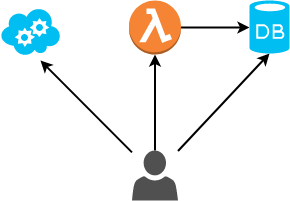
\includegraphics[width=0.5\textwidth]{patterns/thick-client.png}
  \caption{Thick Client}
  \label{fig:patternThickClient}
\end{figure}

\textbf{Solution:} Create thicker, more powerful clients.

Serverless applications, as described in chapter \ref{cha:serverless}, typically rely heavily on third party cloud services (BaaS) interspersed with custom logic in form of serverless functions. In a traditional three-tier web application architecture interaction with these external services would be handled by a server application that sits between the client and the service layers \parencite{robert2016serverlessarchitectures}. Following this model, the client can be limited in functionality whereas the server application plays a larger role. \textcite{sbarski2017serverless} point out that the model of the backend as a gatekeeper between client and services is in conflict with the serverless paradigm. First of all, using FaaS as a middle layer in front of cloud resources directly translates into extra costs: on top of paying for the cloud service call, one has to pay for function invocation and execution for the duration of the network call as well as data transfer between the service and the FaaS provider. Secondly, a middle layer of FaaS results into extra network hops which increases latency and reduces user experience. \textcite{sbarski2017serverless} thus advise against routing everything through a FaaS layer, and advocate building thick clients that communicate directly with cloud services and orchestrate workflows between them.

In addition to the cost benefit, a thicker client has the advantage of improved changeability and separation of concerns, as the single monolithic backend application is replaced by isolated and self-contained components. Doing away with the central arbiter of a server application does come with its trade-offs, including a need for distributed monitoring and further reliance on the security of the cloud services. Importantly not all functionality can or should be moved to the client: security, performance or consistency requirements among others can necessitate a server-side implementation. \parencite{robert2016serverlessarchitectures}.

The Thick Client pattern depends on fine-grained, distributed, request-level authentication in lieu of a gatekeeper server application. This follows naturally from the way serverless functions operate: being stateless and continuously scaling up and down, maintaining a session between the backend and the cloud services is infeasible. Instead of automatically trusting all requests originating from the backend, each cloud service request has to be individually authorized. From a cloud service's point of view, requests originating from a serverless function or directly from the client are both equally untrusted. Hence in serverless architectures, skipping the backend layer is preferable whenever a direct connection between client and services is possible. The Valet Key pattern in section \ref{subsec:valetKey} describes one example of a request-level authentication mechanism. \parencite{adzic2017serverless}

\section{Event patterns} \label{sec:eventPatterns}

Event patterns deal with workflows that are triggered by external events and processed on-demand and asynchronously. FaaS platforms are a good fit for event-driven workflows as they offer integrations to a wide range of event sources as well as non-blocking invocation methods.

\subsection{Event Processor} \label{subsec:Eventprocessing}

\textbf{Problem:} How to execute a task on-demand upon event occurrence?

\begin{figure}[h]
  \centering
  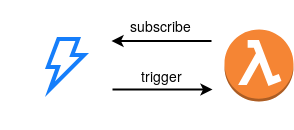
\includegraphics[width=0.45\textwidth]{patterns/event-processor2.png}
  \caption{Event Processor}
  \label{fig:patternEventProcessor}
\end{figure}

\textbf{Solution:} Subscribe a serverless function to a cloud event such as file upload or database change.

The Event Processor pattern consists of subscribing a serverless function to a cloud event source so that when the event occurs, the subscribed function gets invoked with the event context as a parameter \parencite{hong18securingviaserverlesspatterns}. Serverless platforms typically offer a number of integration points to events that originate from various other platform services. For example AWS Lambda functions can be triggered by file uploads, database change events, message queue and notification services, IoT events and others \parencite{awslambda0218}.

\textcite{baldini17currentTrends} mention thumbnail generation triggered by image upload as an exemplary use case of serverless event processing: a bursty, compute-intensive task triggered on-demand by a cloud event. A traditional approach would be to implement a poller system that regularly checks for new images and generates thumbnails as images are detected. Such a system would require constant operation, and depending on polling interval the design leads to either extra network traffic or potentially long delay between event occurrence and processing. The design is especially wasteful in cases where new images come in infrequently. The Event Processor pattern, in turn, can bring considerable cost benefit in case of infrequent or irregular workflows as computation is only ran when necessary \parencite{hong18securingviaserverlesspatterns}. Another advantage is scalability, as functions are automatically invoked as per the number of events: a large number of events occurring at once leads to a similarly large number of serverless functions executing in parallel \parencite{hong18securingviaserverlesspatterns}.

The Event Processor has two counterparts among SOA patterns. In terms of scalability, a serverless Event Processor essentially implements the Service Instance pattern which involves ``deploying multiple instances of service business logic'' to address increased service load. Aptly, the Service Instance pattern is ``best suited for stateless service implementations''. Another related SOA pattern is the Inversion of Communications in which services eschew point-to-point communication in favour of event-driven architecture to reduce coupling between event sources and consumers. The pattern's downsides include the added complexity of designing a system as events and the difficulty of debugging complex event chains. \parencite{rotem12soa}

The Event Processor can also be seen as a serverless form of the Event-Driven Consumer EIP pattern: a message consumer that sits dormant with no active threads until invoked by the messaging system. In essence, the pattern bridges the gap between external events and application-specific callbacks. A notable feature of an Event-Driven Consumer is that it automatically consumes messages as soon as they become available, which in effect means that the consumer has no control on its consumption rate: see the Polling Event Processor in section \ref{subsec:PollingEventProcessor} for an alternative solution. \parencite{hohpe2004enterprise}

Another point to keep in mind when implementing the Event Processor pattern is that some cloud event sources operate in at-least-once message delivery semantics: due to the highly distributed and eventually consistent nature of cloud platforms, events are guaranteed to be triggered at least once, not exactly once \parencite{awslambda0218}. This means that the triggered serverless function should in effect act idempotently, i.e. multiple executions with the same context should result in identical side effects. \textcite{hohpe2004enterprise} introduce a similar concept with the Idempotent Receiver pattern, a listener that can ``safely receive the same message multiple times''. The authors introduce two primary means for achieving idempotency: either explicit deduplication at the receiving end, or defining message semantics to support idempotency. The first approach calls for keeping track of the messages received thus far and ignoring any duplicates among incoming messages, leaving us with the problem of where and for how long to store the message history. The alternative approach is to design messages themselves in a way that ``resending the message does not impact the system'': for example \textit{set account balance to \$10} instead of \textit{increase account balance by \$1}.

\subsection{Periodic Invoker} \label{subsec:periodicInvocation}

\textbf{Problem:} How to execute a task periodically in predefined intervals?

\begin{figure}[h]
  \centering
  
\includegraphics[width=0.4\textwidth]{patterns/periodic-invocation.png}
  \caption{Periodic Invoker}
  \label{fig:patternPeriodicInvocation}
\end{figure}

\textbf{Solution:} Subscribe a serverless function to a scheduler.

This pattern represents an arrangement where a serverless function is invoked periodically by a scheduler, akin to a cron task in Unix-based systems. First, the scheduler invokes the subscribed function according to its configuration. Second, the function carries out its task. Finally, after execution the function can report execution result out to a notification channel, store it in database or shut down if we're not interested in the outcome. The pattern is both conceptually simple and easy to implement, as all the major serverless providers offer integration to a cloud-based scheduler such as AWS CloudWatch Events \parencite{awslambda0218}. Potential use cases include periodical backups, compliance checks, service health checks, database cleanup tasks and other background jobs that are not latency-critical. \parencite{hong18securingviaserverlesspatterns}

\subsection{Polling Event Processor} \label{subsec:PollingEventProcessor}

\textbf{Problem:} How to react to a state change in an external service that doesn't offer an event source?

\begin{figure}[h]
  \centering
  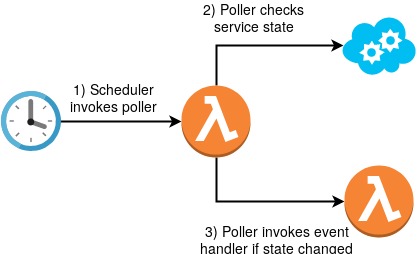
\includegraphics[width=0.4\textwidth]{patterns/polling-event-processor.png}
  \caption{Polling Event Processor}
  \label{fig:PollingEventProcessor}
\end{figure}

\textbf{Solution:} Use the Periodic Invoker pattern to create a polling event processor.

The Event Processor pattern (section \ref{subsec:Eventprocessing}) is used to perform a task in reaction to some state change in another system. The pattern depends on the external system to actively invoke the subscribed function when said state change occurs. Not all systems however are capable of performing such callbacks on state changes, which renders the pattern infeasible in some cases. To work around this limitation we can combine the Event Processor and Periodic Invoker patterns (section \ref{subsec:periodicInvocation}) to essentially implement an event-driven integration point in front of a service where no such event source originally exists. The Polling Event Consumer pattern consists of a Periodic Invoker that repeatedly checks the state of another service and performs a task when found state matches some condition. The task performed can be either implemented in the polling function itself or separated to another function that the poller invokes.

The Polling Event Processor is equivalent to the EIP pattern of Polling Consumer, where a receiver synchronously polls for a message, processes it and then polls for another. As well as offering eventful integration to non-eventful services, the pattern has the advantage of controlling its consumption rate. Whereas the Event Processor executes tasks as soon as events occur, the Polling Event Processor explicitly polls for new events when it is ready for them. The polling interval can also be configured to implement batching. As a downside, a sparse polling interval leads to increased latency between event occurrence and task execution. On the other hand a more fine-grained polling interval results in wasted resources when there are no events to consume. In short, ``polling enables the client to control the rate of consumption, but wastes resources when there’s nothing to consume.'' \parencite{hohpe2004enterprise}

\subsection{Event Broadcast} \label{subsec:EventBroadcast}

\textbf{Problem:} How to invoke multiple parallel functions as a result of a single event occurrence?

% TODO visualize
% \begin{figure}[h]
%   \centering
%   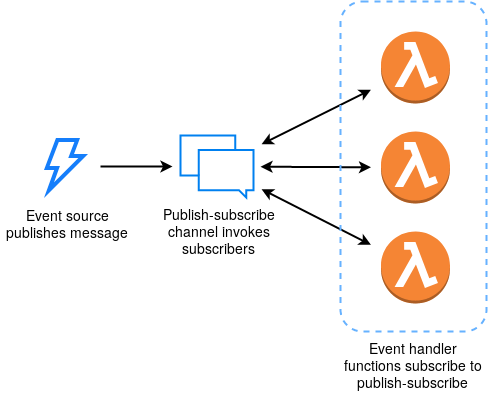
\includegraphics[width=0.4\textwidth]{patterns/event-broadcast.png}
%   \caption{Event Broadcast}
%   \label{fig:eventBroadcast}
% \end{figure}

\textbf{Solution:} Subscribe multiple functions to a notification service, publish notification on event occurrence.

The Event Processor pattern \ref{subsec:Eventprocessing} is applicable within cases of a 1-to-1 relationship between events and tasks, as exemplified above with image upload triggering thumbnail generation. However in other cases a single event can result in multiple independent tasks. For example the image upload event could as well trigger a database update and a notification email, adding up to three self-contained and parallel tasks. Most event sources only support invoking one function per event which leaves us with a couple of options. First, we could set up a new function that subscribes to the image upload event and in turn asynchronously invokes any number of processor functions, as a sort of a parallel Routing Function \label{subsec:routingFunction}. This approach comes with the operational overhead of needing to set up and maintain an additional function per each event broadcast. An alternative solution is to utilize a publish-subscribe channel such as the AWS Simple Notification Service \parencite{awslambda0218}. The key feature of a publish-subscribe channel is that any number of listeners can subscribe to a single channel, which can be used to overcome the 1-to-1 relationship between event sources and functions. Now instead of subscribing a function directly to an event source, functions subscribe to a message channel that the event source publishes a message to upon event occurrence. In addition to achieving parallel fan-out to multiple functions, the pattern has the added benefit of loosed coupling between event sources and handler functions. \parencite{sbarski2017serverless}

The Event Broadcast is derived from the Publish-Subscribe Channel EIP pattern \parencite{hohpe2004enterprise} and the Observer OOP pattern \parencite{gamma94designPatterns}.

\section{API patterns} \label{sec:apiPatterns}

Integrating with external systems.

\subsection{API Composition} \label{subsec:apiComposition}

Hide multiple API calls under a single function.

\subsection{API Aggregation} \label{subsec:apiAggregation}

Hide a sequential multi-step API call under a single function.

\subsection{API Async} \label{subsec:apiAsync}

Turn a synchronized API into an async one.

Request/Reaction SOA \parencite{rotem12soa}.

\subsection{Legacy API Proxy/Staged migration} \label{subsec:legacyApi}

Replace a legacy API with a new one step by step, a.k.a. Strangler \parencite{microsoft18cloudPatterns}.

% \subsection{Separate FaaS handler from core logic} \label
% {subsec:separateHandler}

% Separate FaaS handler core logic in code level.

\section{Data management/access patterns} \label{sec:dataManagementPatterns}

Managing state and accessing external resources.

\subsection{Externalized State} \label{subsec:externalizedState}

Store function state in external storage.

\subsection{Valet Key} \label{subsec:valetKey}

Sign tokens for clients to directly access resources.

\subsection{Least privilege IAM role} \label{subsec:LeastprivilegeIAMrole}

Minimize attack surface by reducing function access roles to bare minimum.

\section{Performance and scalability patterns} \label{sec:perfPatterns}

Address FaaS performance issues.

\subsection{Function Warmer} \label{subsec:FunctionWarmer}

Ping a function intermittently to avoid cold starts.

\subsection{Oversized function} \label{subsec:OversizedFunction}

Choose maximum memory allocation to access faster CPU resources and improve cold start latency.

\subsection{Singleton} \label{subsec:Singleton}

Take advantage of function execution context to avoid reinitializing function dependencies.

\section{Resiliency and availability patterns} \label{sec:resiliencyPatterns}

Maximize serverless system resiliency.

\subsection{Bulkhead} \label{subsec:Bulkhead}

Isolate high-latency code into separate functions to avoid resource contention.

\subsection{Flow control/throttling} \label{subsec:Flow control/throttling}

Throttle invocations to avoid DDoSing yourself.

\subsection{Circuit breaker} \label{subsec:Circuit breaker}

Keep track of component availability to avoid cascading failures.

